\chapter{RESULTADOS E DISCUSSÃO}

Neste item serão apresentados os resultados obtidos do presente trabalho.

\section{FERRAMENTA COMPUTACIONAL INTENSIO}

As páginas da interface gráfica ficaram divididas entre as abas iniciais, e a barra de ferramentas.

\subsection{As abas da ferramenta}

A interface gráfica ficou dividida em três abas. A primeira e principal delas têm o nome de \textbf{Equações do Mapa} e mostra o mapa interativo da Paraíba, que como explicado anteriormente, permite o cálculo da equação IDF através da escolha de uma coordenada ao clicar no mapa, por meio de interpolação. Também é possível apenas escolher uma das cidades paraibanas contida na lista. Tudo isso pode ser visto na Figura 5.1.\bigskip

\begin{figure}[!ht]
	\centering
	\caption{Aba "Equações do Mapa".}
	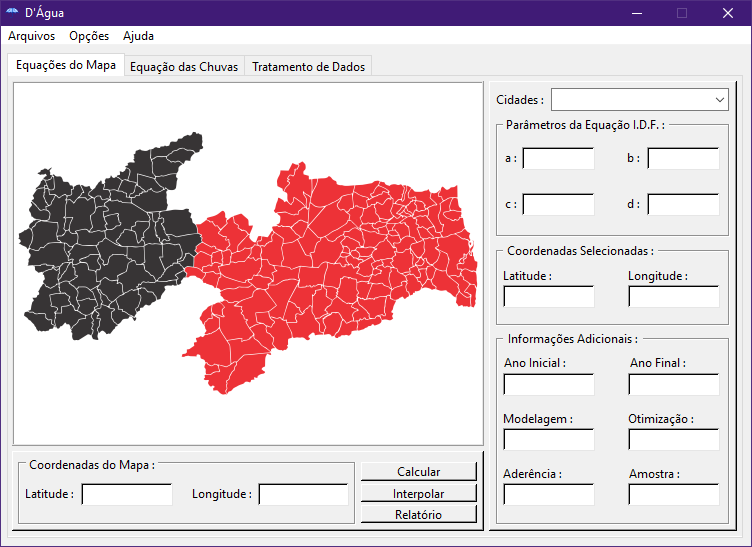
\includegraphics[width=.7625\linewidth]{figuras/equacoes_do_mapa.png}
	\caption*{\textbf{Fonte:} De autoria própria (2023).}
	\label{fig:equacoes_do_mapa.png}
\end{figure}

 A segunda aba é chamada de \textbf{Equação das Chuvas} e envolve os cálculos da equação IDF com base nos dados de séries temporais inseridos pelo usuário. Nela também é possível configurar as durações, tempos de retorno e métodos usados tanto nos cálculos citados anteriormente, como nos da primeira aba que utilizam as precipitações do banco de dados. Ou seja, suas configurações afetam toda a ferramenta e podem ser vistas na Figura 5.2.

\begin{figure}[!ht]
	\centering
	\caption{Aba "Equação das Chuvas".}
	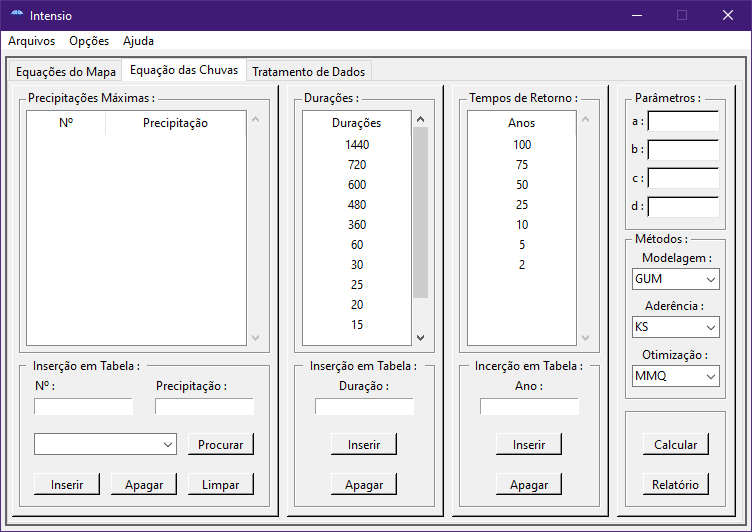
\includegraphics[width=.7625\linewidth]{figuras/equacao_das_chuvas.png}
	\caption*{\textbf{Fonte:} De autoria própria (2023).}
	\label{fig:equacao_das_chuvas.png}
\end{figure}

Observa-se a terceira e última aba na Figura 5.3, chamada de \textbf{Tratamento de Dados}, ela envolve o tratamento de séries históricas de precipitações diárias, resultando nas máximas diárias anuais, que podem ser exportadas para o cálculo da equação IDF na segunda aba.\bigskip

\begin{figure}[!ht]
	\centering
	\caption{Aba "Tratamento de Dados".}
	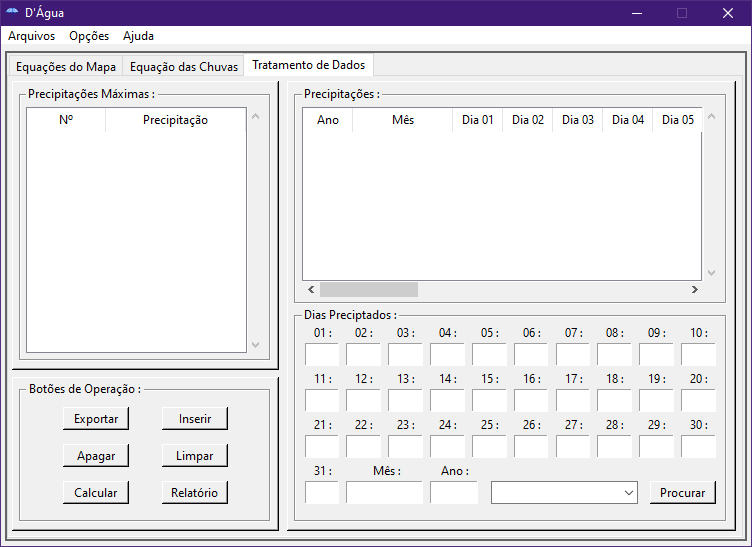
\includegraphics[width=.7625\linewidth]{figuras/tratamento_de_dados.png}
	\caption*{\textbf{Fonte:} De autoria própria (2023).}
	\label{fig:tratamento_de_dados.png}
\end{figure}

\newpage

\subsection{A barra de ferramentas}

A primeira ferramenta da barra é chamada \textbf{Arquivos}, e nela há a possibilidade de reiniciar ou apenas sair do programa. Já em \textbf{Opções} é possível acessar o \textbf{Banco de Dados}, \textbf{Configurações} e \textbf{Varreduras}.

O item  \textbf{Banco de Dados} contém as informações de precipitações diárias das cidades da Paraíba, que são usados no desenvolvimento do método de preenchimento de falhas por interpolação IDW nos cálculos do mapa paraibano e da lista de cidades. Também é possível exportar os dados da cidade escolhida para a aba de tratamento de dados ou salva-los na própria máquina do usuário, no formato de texto ou \textit{Comma-Separated-Values} (CSV).\bigskip

\begin{figure}[!ht]
	\centering
	\caption{Banco de dados da ferramenta Opções.}
	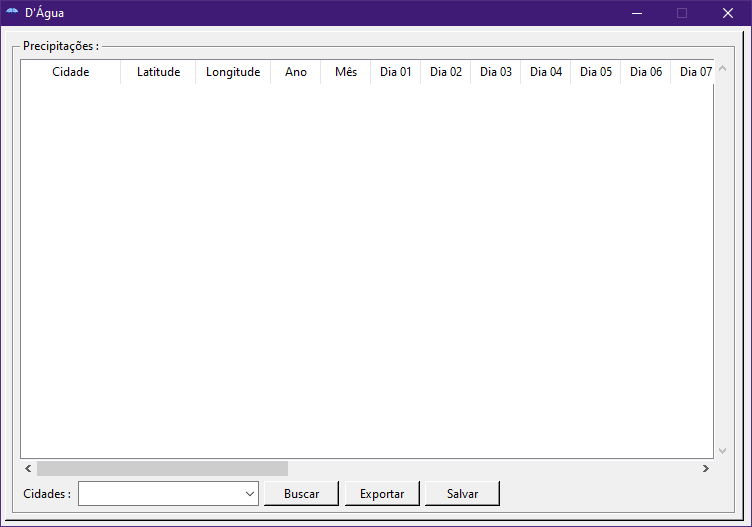
\includegraphics[width=.7625\linewidth]{figuras/banco_de_dados.png}
	\caption*{\textbf{Fonte:} De autoria própria (2023).}
	\label{fig:banco_de_dados.png}
\end{figure}

Já o item \textbf{Configurações} possibilita ao usuário definir manualmente algumas informações que são usadas nos cálculos. Seguindo pela ordem, é possível escolher entre coeficientes próprios de desagregação ou os estabelecidos pela DAEE/CETESB (1980), e a porcentagem de aderência usada no cálculo da equação IDF.

Também é possível decidir a quantidade de dias que representará o limiar de falhas usado na terceira aba, as otimizações de modelagem, aderência e otimização que caso ativados buscarão sempre os métodos que resultam em mais precisão nos parâmetros da equação IDF gerada. Por fim há a possibilidade de selecionar a quantidade de iteração que o algoritmo fará durante o uso dos métodos de otimização no cálculo dos parâmetros da equação. É importante salientar que o mau uso dessas ferramentas pode exigir altos níveis de processamento da máquina devido a quantidade de iterações. Observa-se na Figura 5.5 a página de configurações.

\newpage

\begin{figure}[!ht]
	\centering
	\caption{Configurações da ferramenta Opções.}
	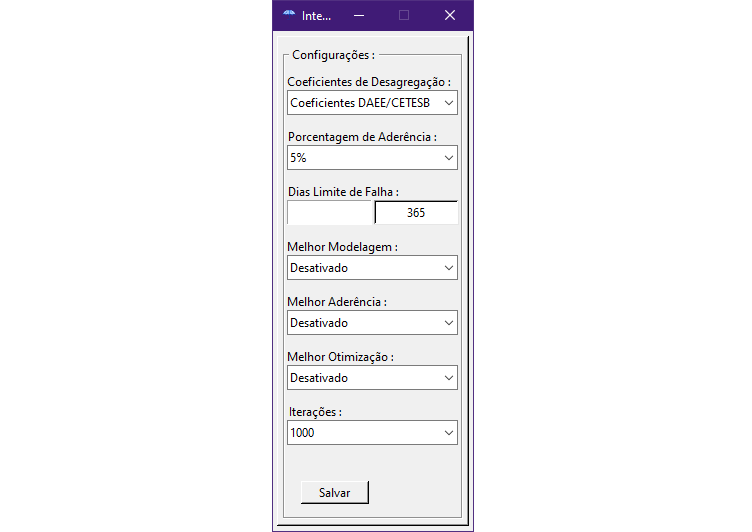
\includegraphics[width=.7615\linewidth]{figuras/configuracoes.png}
	\caption*{\textbf{Fonte:} De autoria própria (2023).}
	\label{fig:figuras/configuracoes.png}
\end{figure}

O item \textbf{Varreduras} pode ser vista na Figura 5.6. Ela permite ao usuário alterar os números de partida ou intervalos dos métodos de otimização. Bons ajustes manuais dos mesmos pode resultar em uma melhora na precisão das equações geradas, em contrapartida o mau uso pode diminuir as porcentagens de acurácia ou até mesmo inviabilizar o cálculo.\bigskip

\begin{figure}[!ht]
	\centering
	\caption{Varreduras da ferramenta Opções.}
	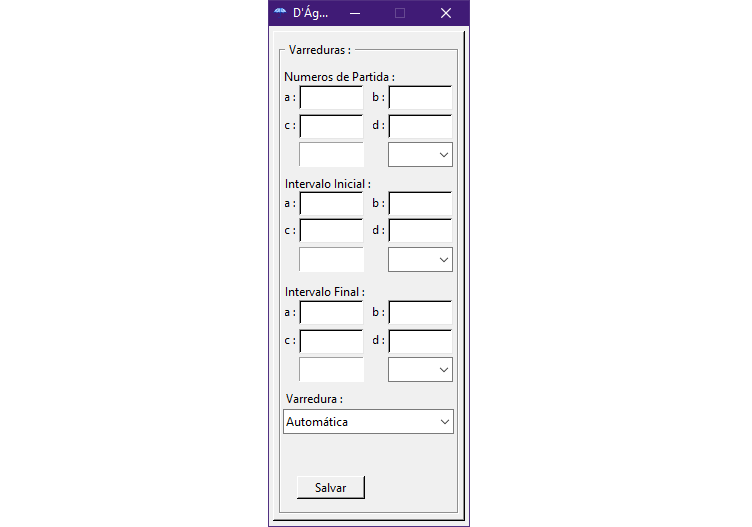
\includegraphics[width=.7615\linewidth]{figuras/varreduras.png}
	\caption*{\textbf{Fonte:} De autoria própria (2023).}
	\label{fig:figuras/varreduras.png}
\end{figure}

\newpage

A última ferramenta é a de \textbf{Ajuda}, e nela tem-se os itens para auxílio do usuário. Em \textbf{Estudo} aborda-se o presente trabalho como visto na Figura 5.7.

\begin{figure}[!ht]
	\centering
	\caption{Estudo da ferramenta Ajuda.}
	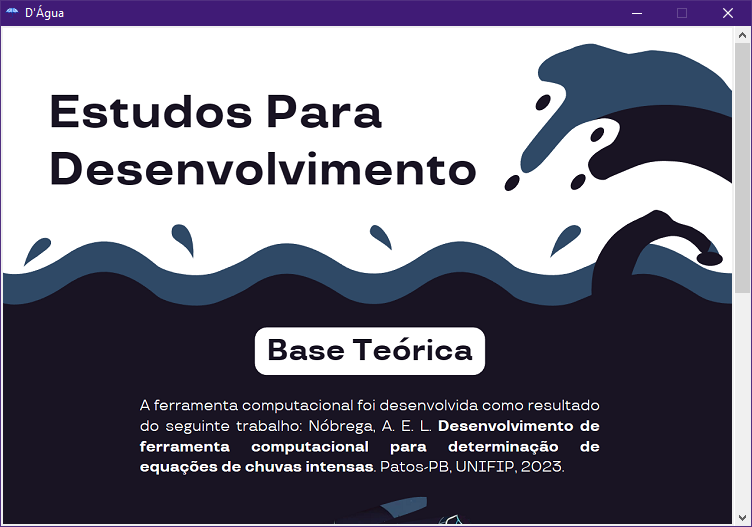
\includegraphics[width=.7625\linewidth]{figuras/estudo.png}
	\caption*{\textbf{Fonte:} De autoria própria (2023).}
	\label{fig:figuras/estudo.png}
\end{figure}

Já o item \textbf{Ferramenta} explica como funciona a inserção de dados e os cálculos computacionais, observado na Figura 5.8.

\begin{figure}[!ht]
	\centering
	\caption{Ferramenta da ferramenta Ajuda.}
	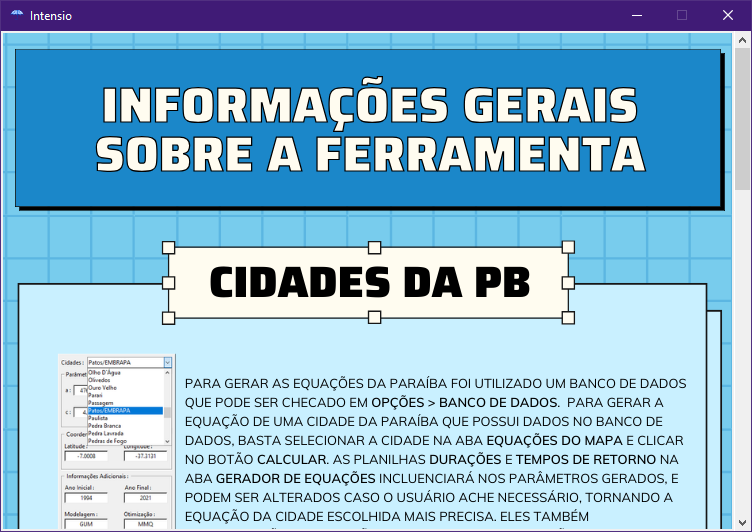
\includegraphics[width=.7625\linewidth]{figuras/ferramenta.png}
	\caption*{\textbf{Fonte:} De autoria própria (2023).}
	\label{fig:figuras/ferramenta.png}
\end{figure}

\newpage

O item \textbf{Manual} abre um arquivo no formato \textit{Portable Document Format} (PDF) fora da ferramenta, que contém um manual de uso prático da ferramenta, como na Figura 5.9.

\begin{figure}[!ht]
	\centering
	\caption{Manual da ferramenta Ajuda.}
	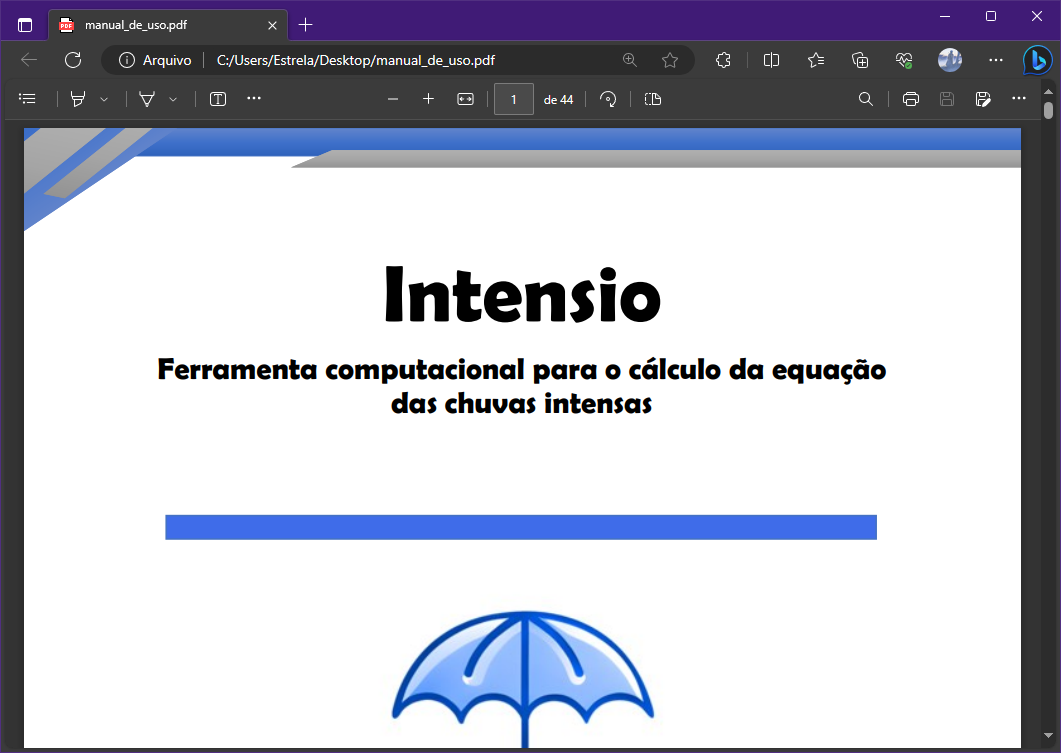
\includegraphics[width=.7625\linewidth]{figuras/manual.png}
	\caption*{\textbf{Fonte:} De autoria própria (2023).}
	\label{fig:figuras/manual.png}
\end{figure}

Por último, a ferramenta \textbf{Ajuda} possui o item \textbf{Siglas} que trata das abreviaturas utilizadas, visível na Figura 5.10.

\begin{figure}[!ht]
	\centering
	\caption{Siglas da ferramenta Ajuda.}
	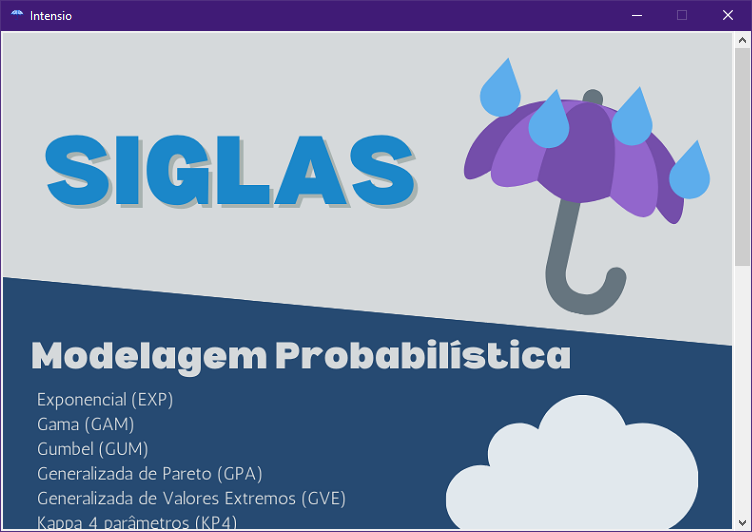
\includegraphics[width=.7625\linewidth]{figuras/siglas.png}
	\caption*{\textbf{Fonte:} De autoria própria (2023).}
	\label{fig:figuras/siglas.png}
\end{figure}

\newpage

\section{VALIDAÇÃO DAS EQUAÇÕES GERADAS}

A validação das equações, trata-se da análise da acurácia destas após geradas. Sempre que o usuário submeter dados, escolher uma coordenada do mapa ou cidade da lista e calcular os parâmetros da equação IDF, será gerado um relatório que pode ser acionado ao clicar no botão de mesmo nome, e visto tanto na Figura 5.1 como na Figura 5.2. Neles, estão contidos os testes de NS e RMSE, que informam quão precisos estão os parâmetros em relação às curvas IDF qual eles foram calculados.

É importante notar que cada equação será analisada individualmente, cabendo ao calculista decidir de acordo com os testes feitos, se ele está satisfeito com a precisão dos parâmetros gerados. Outra observação importante a se fazer é a de que, os testes de acurácia analisam apenas se os parâmetros calculados estão precisos em relação aos dados observados, logo, cabe ao usuário discernir se as séries históricas que ele está informando representam bem a realidade.

É possível salvar o relatório gerado em um arquivo de texto, que informa a representação da equação IDF, um resumo de todo o processo de cálculo feito junto de todas as variáveis calculadas e uma tabela com intensidades calculadas a partir da equação gerada, utilizando as durações e tempos de retorno informados no início do cálculo. Visualiza-se a página do relatório na Figura 5.11.\bigskip

\begin{figure}[!ht]
	\centering
	\caption{Relatório dos parâmetros da equação IDF.}
	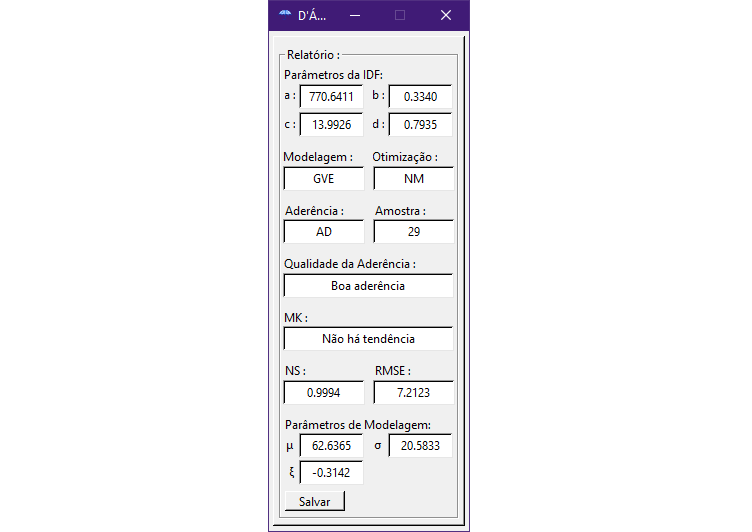
\includegraphics[width=.7625\linewidth]{figuras/relatorio_de_equacoes.png}
	\caption*{\textbf{Fonte:} De autoria própria (2023).}
	\label{fig:figuras/relatorio_de_equacoes.png}
\end{figure}

\newpage

Existe também um relatório para o tratamento de dados que é acionado pelo botão de nome similar visto na Figura 5.3. Nele consegue-se analisar a quantidade de dias totais e faltantes, além da porcentagem de erros geral obtido, e anual permitido de acordo com o limiar de falhas informado. Também é possível salvar esse relatório em um arquivo de texto que contém as informações do tratamento de dados e uma tabela com as precipitações máximas diárias anuais geradas, e os dias faltantes de cada ano. Observa-se a página do relatório na Figura 5.12.\bigskip

\begin{figure}[!ht]
	\centering
	\caption{Relatório de falhas do tratamento de dados.}
	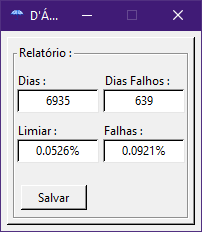
\includegraphics[width=.21\linewidth]{figuras/relatorio_de_falhas.png}
	\caption*{\textbf{Fonte:} De autoria própria (2023).}
	\label{fig:figuras/relatorio_de_falhas.png}
\end{figure}

\section{DISPONIBILIZAÇÃO DA FERRAMENTA}

Como resultado final, foi disponibilizado por Nóbrega (2023) o acesso ao repositório do código fonte no GitHub, com todos os algoritmos criados no desenvolvimento da ferramenta. Nóbrega (2023) também disponibilizou o caminho para transferência do manual de uso prático da ferramenta no formato PDF, e do instalador da ferramenta computacional, de forma a facilitar o seu acesso.\bigskip

\section{EQUAÇÕES GERADAS ATRAVÉS DA FERRAMENTA}

Como foi explicado anteriormente, a ferramenta possui dados de precipitação que compreendem todo o estado da Paraíba, que podem servir como modelo para posteriores inserções de dados de outras regiões. E para comprovar o pleno funcionamento da ferramenta, foram geradas equações para todas as cidades presentes no banco de dados. 

Foi utilizado o método de otimização NM, e o teste de aderência de KS para um nível de significância de cinco por cento, otimizando apenas as distribuições probabilísticas. Foram geradas com sucesso um total de equações para 226 cidades, de um total de 242, vistas na Tabela 5.1.\bigskip

\newpage

% Primeira parte da tabela

\begin{table}[ht]
\centering
\caption{Equações IDF da Paraíba geradas através de ferramenta Intensio}
\captionsetup{justification=raggedleft,singlelinecheck=false}
\caption*{(Continua)}
\small
\begin{tabular}{ccccccccc}
\hline
\textbf{Cidade} & \textbf{Am.} & \textbf{a} & \textbf{b} & \textbf{c} & \textbf{d} & \textbf{NS} & \textbf{RMSE} & \textbf{Md.} \\ \hline
Agua Branca & 29 & 703,8389 & 0,1648 & 9,7910 & 0,7244 & 0,9980 & 8,8084 & NOG \\
Aguiar & 29 & 840,3493 & 0,1488 & 9,7910 & 0,7244 & 0,9994 & 5,4523 & NOG \\
Alagoa Grande & 29 & 566,1002 & 0,2063 & 9,7910 & 0,7244 & 0,9991 & 5,4753 & GVE \\
Alagoa Nova & 29 & 663,6596 & 0,1825 & 9,7910 & 0,7244 & 0,9976 & 9,6962 & LOG \\
Alagoinha & 29 & 592,6732 & 0,2387 & 9,7910 & 0,7244 & 0,9991 & 6,6931 & GVE \\
Alcantil & 23 & 504,2508 & 0,2199 & 9,7910 & 0,7244 & 0,9967 & 10,0432 & LN2 \\
Algodão de Jandaíra & 29 & 499,3560 & 0,1772 & 9,7910 & 0,7244 & 0,9973 & 7,6612 & LOG \\
Alhandra & 29 & 956,9647 & 0,1718 & 9,7910 & 0,7244 & 0,9980 & 12,3251 & LOG \\
Amparo & 25 & 816,4717 & 0,1923 & 9,7910 & 0,7244 & 0,9969 & 14,2015 & LOG \\
Araçagi & 29 & 661,5735 & 0,1589 & 9,7910 & 0,7244 & 0,9984 & 7,1774 & NOG \\
Arara & 27 & 452,5077 & 0,2509 & 9,7910 & 0,7244 & 0,9989 & 5,7949 & GVE \\
Araruna & 29 & 631,8274 & 0,1833 & 9,7910 & 0,7244 & 0,9977 & 9,1662 & NOG \\
Areia & 29 & 725,5098 & 0,1723 & 9,7910 & 0,7244 & 0,9980 & 9,3919 & LOG \\
Areia de Baraúnas & 13 & 630,2953 & 0,2054 & 9,7910 & 0,7244 & 0,9984 & 8,2205 & PT3 \\
Areial & 29 & 474,7496 & 0,1860 & 9,7910 & 0,7244 & 0,9981 & 6,2811 & GVE \\
Aroeiras & 29 & 473,3835 & 0,2400 & 9,7910 & 0,7244 & 0,9973 & 9,2688 & GVE \\
Assunção & 18 & 698,5792 & 0,1658 & 9,7910 & 0,7244 & 0,9980 & 8,8233 & LOG \\
Baía da Traição & 28 & 856,8386 & 0,2563 & 9,7910 & 0,7244 & 0,9997 & 6,1284 & GVE \\
Bananeiras & 29 & 680,1219 & 0,1704 & 9,7910 & 0,7244 & 0,9980 & 8,6129 & LOG \\
Baraúna & 17 & 546,7797 & 0,2192 & 9,7910 & 0,7244 & 0,9969 & 10,5098 & GVE \\
Barra de Santa Rosa & 29 & 471,2786 & 0,2675 & 9,7910 & 0,7244 & 0,9963 & 12,1375 & GVE \\
Barra de Santana & 27 & 445,1012 & 0,2311 & 9,7910 & 0,7244 & 0,9988 & 5,5923 & NOG \\
Barra de São Miguel & 29 & 607,0755 & 0,1917 & 9,7910 & 0,7244 & 0,9973 & 9,8449 & NOG \\
Bayeux & 27 & 987,0451 & 0,1722 & 9,7910 & 0,7244 & 0,9978 & 13,4115 & LOG \\
Belém & 29 & 657,9642 & 0,2119 & 9,7910 & 0,7244 & 0,9970 & 12,1619 & GVE \\
\begin{tabular}[c]{@{}c@{}}Belém do \\ Brejo do Cruz\end{tabular} & 29 & 672,7598 & 0,2550 & 9,7910 & 0,7244 & 0,9985 & 10,4801 & GVE \\
Bernardino Batista & 19 & 620,3196 & 0,2526 & 9,7910 & 0,7244 & 0,9997 & 3,9738 & GVE \\
Boa Ventura & 29 & 895,9545 & 0,1747 & 9,7910 & 0,7244 & 0,9979 & 11,9447 & LOG \\
Boa Vista & 29 & 484,3072 & 0,2989 & 9,7910 & 0,7244 & 0,9958 & 15,1673 & LN2 \\
Bom Jesus & 28 & 828,9001 & 0,1604 & 9,7910 & 0,7244 & 0,9984 & 9,0966 & NOG \\
Bom Sucesso & 29 & 712,0361 & 0,1580 & 9,7910 & 0,7244 & 0,9984 & 7,7784 & LOG \\
\begin{tabular}[c]{@{}c@{}}Boqueirão/\\ Açude Boqueirão\end{tabular} & 29 & 489,3461 & 0,2922 & 9,7910 & 0,7244 & 0,9969 & 12,7641 & GVE \\ 
Borborema & 27 & 686,2451 & 0,1794 & 9,7910 & 0,7244 & 0,9976 & 9,8761 & LOG \\
Brejo do Cruz & 29 & 779,4120 & 0,1945 & 9,7910 & 0,7244 & 0,9971 & 13,0705 & LOG \\
Brejo dos Santos & 29 & 735,2317 & 0,1669 & 9,7910 & 0,7244 & 0,9981 & 8,9273 & LOG \\
Cabaceiras & 29 & 478,3793 & 0,3120 & 9,7910 & 0,7244 & 0,9985 & 9,4610 & NOG \\
Cabedelo & 20 & 1041,7680 & 0,1636 & 9,7910 & 0,7244 & 0,9971 & 15,6854 & LOG \\
\begin{tabular}[c]{@{}c@{}}Cachoeira \\ dos Índios\end{tabular} & 28 & 766,6130 & 0,1314 & 9,7910 & 0,7244 & 0,9984 & 7,6301 & LOG \\
Cacimba de Areia & 29 & 775,8838 & 0,1955 & 9,7910 & 0,7244 & 0,9988 & 8,4599 & NOG \\
Cacimba de Dentro & 29 & 569,2094 & 0,1954 & 9,7910 & 0,7244 & 0,9974 & 9,0670 & GVE \\
Cacimbas & 19 & 855,6570 & 0,1751 & 9,7910 & 0,7244 & 0,9969 & 13,8633 & LOG \\
Caiçara & 29 & 547,5272 & 0,2155 & 9,7910 & 0,7244 & 0,9982 & 7,9850 & GVE \\
Cajazeiras & 29 & 790,2086 & 0,1861 & 9,7910 & 0,7244 & 0,9992 & 6,8471 & NOG \\ \hline
\end{tabular}
\end{table}

\bigskip

\newpage

% Segunda parte da tabela

\begin{table}[ht]
\centering
\caption*{\textbf{\fontsize{10.5}{14}\selectfont Tabela 5.1} - Equações IDF da Paraíba geradas através de ferramenta Intensio}
\captionsetup{justification=raggedleft,singlelinecheck=false}
\caption*{(Continua)}
\small
\begin{tabular}{ccccccccc}
\hline
\textbf{Cidade} & \textbf{Am.} & \textbf{a} & \textbf{b} & \textbf{c} & \textbf{d} & \textbf{NS} & \textbf{RMSE} & \textbf{Md.} \\ \hline
\begin{tabular}[c]{@{}c@{}}Cajazeiras/Açude \\ Engenheiro Avidos\end{tabular} & 29 & 825,6586 & 0,1655 & 9,7910 & 0,7244 & 0,9981 & 10,1543 & LOG \\
Cajazeirinhas & 23 & 655,7415 & 0,2815 & 9,7910 & 0,7244 & 0,9997 & 5,4178 & NOG \\
Caldas Brandão & 29 & 715,1540 & 0,1455 & 9,7910 & 0,7244 & 0,9983 & 7,5943 & LOG \\
Camalaú & 29 & 620,1916 & 0,2377 & 9,7910 & 0,7244 & 0,9988 & 8,0736 & GVE \\
\begin{tabular}[c]{@{}c@{}}Campina Grande/\\ EMBRAPA\end{tabular} & 29 & 526,6675 & 0,1845 & 9,7910 & 0,7244 & 0,9975 & 7,8777 & LOG \\
\begin{tabular}[c]{@{}c@{}}Campina Grande/\\ INSA\end{tabular} & 16 & 578,3930 & 0,1928 & 9,7910 & 0,7244 & 0,9965 & 10,7373 & NOG \\
\begin{tabular}[c]{@{}c@{}}Campina Grande/\\ São José da Mata\end{tabular} & 29 & 477,9186 & 0,1887 & 9,7910 & 0,7244 & 0,9984 & 5,8855 & NOG \\
\begin{tabular}[c]{@{}c@{}}Campina Grande/\\ Sítio Açude\\  de Dentro\end{tabular} & 29 & 462,0710 & 0,2822 & 9,7910 & 0,7244 & 0,9995 & 4,7927 & NOG \\
\begin{tabular}[c]{@{}c@{}}Campo de Santana/\\ Tacima\end{tabular} & 28 & 631,4019 & 0,2302 & 9,7910 & 0,7244 & 0,9966 & 13,4106 & LN2 \\
Capim & 19 & 793,4762 & 0,1706 & 9,7910 & 0,7244 & 0,9975 & 11,3880 & LOG \\
Caraúbas & 29 & 530,8617 & 0,2294 & 9,7910 & 0,7244 & 0,9978 & 8,9885 & NOG \\
Carrapateira & 28 & 947,9802 & 0,1706 & 9,7910 & 0,7244 & 0,9974 & 13,7050 & LOG \\
\begin{tabular}[c]{@{}c@{}}Casserengue/\\ Sítio Salgado\end{tabular} & 29 & 440,3983 & 0,1730 & 9,7910 & 0,7244 & 0,9978 & 5,9240 & NOG \\
Catingueira & 29 & 820,9140 & 0,1481 & 9,7910 & 0,7244 & 0,9980 & 9,5153 & NOG \\
Catolé do Rocha & 29 & 674,1147 & 0,2095 & 9,7910 & 0,7244 & 0,9990 & 7,1145 & GVE \\
\begin{tabular}[c]{@{}c@{}}Catolé do Rocha/\\ Escola Técnica\end{tabular} & 29 & 744,9367 & 0,1482 & 9,7910 & 0,7244 & 0,9980 & 8,7413 & LOG \\
Caturité & 19 & 475,7168 & 0,2445 & 9,7910 & 0,7244 & 0,9964 & 11,0229 & LN2 \\
\begin{tabular}[c]{@{}c@{}}Caturité/Fazenda \\ Campo de Emas\end{tabular} & 21 & 591,4445 & 0,3057 & 9,7910 & 0,7244 & 0,9957 & 19,1822 & LN2 \\
Conceição & 29 & 739,5461 & 0,1366 & 9,7910 & 0,7244 & 0,9985 & 7,2430 & LOG \\
Condado & 29 & 748,9526 & 0,2358 & 9,7910 & 0,7244 & 0,9987 & 10,1404 & GVE \\
Conde & 22 & 993,2376 & 0,1672 & 9,7910 & 0,7244 & 0,9977 & 13,3432 & LOG \\
\begin{tabular}[c]{@{}c@{}}Conde/Açude \\ Gramame Mamuaba\end{tabular} & 28 & 901,5979 & 0,1571 & 9,7910 & 0,7244 & 0,9997 & 4,4141 & NOG \\ 
Congo & 29 & 681,8482 & 0,1807 & 9,7910 & 0,7244 & 0,9983 & 8,2533 & NOG \\
\begin{tabular}[c]{@{}c@{}}Coremas/\\ Açude Coremas\end{tabular} & 29 & 901,9537 & 0,1389 & 9,7910 & 0,7244 & 0,9985 & 8,7597 & NOG \\
Coxixola & 29 & 774,2229 & 0,2616 & 9,7910 & 0,7244 & 0,9962 & 19,8017 & LN2 \\
Cubati & 27 & 512,7133 & 0,2726 & 9,7910 & 0,7244 & 0,9960 & 13,9494 & LN2 \\
Cuité & 29 & 624,0487 & 0,2149 & 9,7910 & 0,7244 & 0,9992 & 6,0603 & NOG \\
\begin{tabular}[c]{@{}c@{}}Cuité de \\ Mamanguape\end{tabular} & 18 & 877,7301 & 0,2070 & 13,9926 & 0,7935 & 0,9964 & 12,0965 & GUM \\ 
Cuitegi & 22 & 649,3738 & 0,1590 & 9,7910 & 0,7244 & 0,9969 & 9,8508 & LOG \\
Curral de Cima & 18 & 725,6193 & 0,1773 & 9,7910 & 0,7244 & 0,9977 & 10,2991 & LOG \\
Curral Velho & 28 & 741,2223 & 0,1662 & 9,7910 & 0,7244 & 0,9998 & 3,2738 & NOG \\
Damião & 23 & 420,0738 & 0,3036 & 9,7910 & 0,7244 & 0,9985 & 7,9805 & GVE \\
Desterro & 29 & 743,9167 & 0,2677 & 9,7910 & 0,7244 & 0,9985 & 12,0680 & GVE \\ \hline
\end{tabular}
\end{table}

\newpage

% Terceira parte da tabela

\begin{table}[ht]
\centering
\caption*{\textbf{\fontsize{10.5}{14}\selectfont Tabela 5.1} - Equações IDF da Paraíba geradas através de ferramenta Intensio}
\captionsetup{justification=raggedleft,singlelinecheck=false}
\caption*{(Continua)}
\small
\begin{tabular}{ccccccccc}
\hline
\textbf{Cidade} & \textbf{Am.} & \textbf{a} & \textbf{b} & \textbf{c} & \textbf{d} & \textbf{NS} & \textbf{RMSE} & \textbf{Md.} \\ \hline
Diamante & 28 & 795,4016 & 0,1625 & 9,7910 & 0,7244 & 0,9978 & 10,2250 & LOG \\
Dona Inês & 29 & 559,9324 & 0,2021 & 9,7910 & 0,7244 & 0,9985 & 7,1063 & GVE \\
Duas Estradas & 27 & 666,7060 & 0,1511 & 9,7910 & 0,7244 & 0,9986 & 6,6822 & LOG \\
Emas & 29 & 764,3276 & 0,1843 & 9,7910 & 0,7244 & 0,9975 & 11,4090 & LOG \\
Esperança & 28 & 556,2148 & 0,1836 & 9,7910 & 0,7244 & 0,9972 & 8,7953 & LOG \\
\begin{tabular}[c]{@{}c@{}}Esperança/\\ São Miguel\end{tabular} & 27 & 465,4854 & 0,2561 & 9,7910 & 0,7244 & 0,9994 & 4,4333 & GVE \\
Fagundes & 29 & 586,3965 & 0,2842 & 9,7910 & 0,7244 & 0,9984 & 10,5983 & GVE \\
Frei Martinho & 27 & 557,2249 & 0,3148 & 9,7910 & 0,7244 & 0,9957 & 18,9249 & LN2 \\
Gado Bravo & 19 & 537,3323 & 0,1663 & 9,7910 & 0,7244 & 0,9985 & 5,8451 & NOG \\
Guarabira & 29 & 691,6546 & 0,1825 & 9,7910 & 0,7244 & 0,9976 & 10,1027 & LOG \\
Gurinhém & 28 & 622,0467 & 0,1848 & 9,7910 & 0,7244 & 0,9975 & 9,3545 & LOG \\
Gurjão & 29 & 660,8858 & 0,2597 & 9,7910 & 0,7244 & 0,9962 & 16,7205 & LN2 \\
Ibiara & 29 & 810,4714 & 0,1772 & 9,7910 & 0,7244 & 0,9973 & 12,4068 & LOG \\
Igaracy & 29 & 948,3099 & 0,1441 & 9,7910 & 0,7244 & 0,9985 & 9,5272 & LOG \\
Imaculada & 29 & 754,1749 & 0,1913 & 9,7910 & 0,7244 & 0,9970 & 12,7834 & LOG \\
Ingá & 29 & 425,3386 & 0,3311 & 9,7910 & 0,7244 & 0,9998 & 3,3805 & GVE \\
Itaporanga & 29 & 930,5906 & 0,1780 & 9,7910 & 0,7244 & 0,9990 & 8,8434 & NOG \\
\begin{tabular}[c]{@{}c@{}}Itaporanga/\\ Fazenda Veludo\end{tabular} & 19 & 852,4966 & 0,2223 & 9,7910 & 0,7244 & 0,9967 & 17,2360 & LN2 \\
Itapororoca & 28 & 764,1475 & 0,1349 & 9,7910 & 0,7244 & 0,9983 & 7,9604 & NOG \\
Itatuba & 28 & 507,5285 & 0,2293 & 9,7910 & 0,7244 & 0,9988 & 6,3528 & NOG \\
Jacaraú & 29 & 726,4185 & 0,1598 & 9,7910 & 0,7244 & 0,9993 & 5,1655 & NOG \\
Jericó & 29 & 686,7858 & 0,1512 & 9,7910 & 0,7244 & 0,9996 & 3,5521 & NOG \\
\begin{tabular}[c]{@{}c@{}}João Pessoa/\\ CEDRES\end{tabular} & 17 & 1076,5964 & 0,1174 & 9,7910 & 0,7244 & 0,9985 & 9,7191 & LOG \\
\begin{tabular}[c]{@{}c@{}}João Pessoa/\\ DFAARA\end{tabular} & 29 & 1267,3979 & 0,1228 & 9,7910 & 0,7244 & 0,9980 & 13,4584 & LOG \\
\begin{tabular}[c]{@{}c@{}}João Pessoa/\\ Mangabeira\end{tabular} & 27 & 1154,5927 & 0,1454 & 9,7910 & 0,7244 & 0,9980 & 13,4466 & LOG \\
João Pessoa/Mares & 27 & 905,2674 & 0,1967 & 9,7910 & 0,7244 & 0,9985 & 11,0486 & GVE \\
\begin{tabular}[c]{@{}c@{}}Joca Claudino/\\ Santarém\end{tabular} & 19 & 694,7098 & 0,1626 & 9,7910 & 0,7244 & 0,9982 & 8,2496 & LOG \\
Juarez Távora & 29 & 605,4752 & 0,1825 & 9,7910 & 0,7244 & 0,9976 & 8,9674 & LOG \\
Juazeirinho & 29 & 649,7521 & 0,1896 & 9,7910 & 0,7244 & 0,9971 & 10,7725 & LOG \\ Junco do Seridó & 29 & 692,0006 & 0,1725 & 9,7910 & 0,7244 & 0,9976 & 9,8063 & LOG \\ Juripiranga & 27 & 698,5518 & 0,2141 & 9,7910 & 0,7244 & 0,9994 & 5,6581 & NOG \\
Juru & 29 & 687,2482 & 0,1587 & 9,7910 & 0,7244 & 0,9984 & 7,5645 & LOG \\
Lagoa & 29 & 746,0658 & 0,1320 & 9,7910 & 0,7244 & 0,9986 & 6,9662 & LOG \\
Lagoa de Dentro & 28 & 616,7919 & 0,1869 & 9,7910 & 0,7244 & 0,9992 & 5,2577 & GVE \\
Lagoa Seca & 28 & 625,3672 & 0,1653 & 9,7910 & 0,7244 & 0,9996 & 3,4406 & NOG \\
Lastro & 28 & 642,9770 & 0,1923 & 9,7910 & 0,7244 & 0,9997 & 3,4302 & NOG \\
Livramento & 29 & 750,6357 & 0,2096 & 9,7910 & 0,7244 & 0,9969 & 13,9866 & LN2 \\
Logradouro & 13 & 604,0265 & 0,1814 & 9,7910 & 0,7244 & 0,9983 & 7,4379 & NOG \\
Lucena & 21 & 1056,1091 & 0,1562 & 9,7910 & 0,7244 & 0,9967 & 16,4472 & LOG \\
Mãe D`Água & 29 & 750,7769 & 0,1418 & 9,7910 & 0,7244 & 0,9987 & 6,8478 & NOG \\ \hline
\end{tabular}
\end{table}

\newpage

% Quarta parte da tabela

\begin{table}[ht]
\centering
\caption*{\textbf{\fontsize{10.5}{14}\selectfont Tabela 5.1} - Equações IDF da Paraíba geradas através de ferramenta Intensio}
\captionsetup{justification=raggedleft,singlelinecheck=false}
\caption*{(Continua)}
\small
\begin{tabular}{ccccccccc}
\hline
\textbf{Cidade} & \textbf{Am.} & \textbf{a} & \textbf{b} & \textbf{c} & \textbf{d} & \textbf{NS} & \textbf{RMSE} & \textbf{Md.} \\ \hline
Manaíra & 29 & 736,3101 & 0,1858 & 9,7910 & 0,7244 & 0,9979 & 10,2482 & GVE \\
Mari & 27 & 749,8562 & 0,1482 & 9,7910 & 0,7244 & 0,9983 & 8,1166 & LOG \\
Marizópolis & 22 & 778,8124 & 0,1621 & 9,7910 & 0,7244 & 0,9983 & 8,9234 & LOG \\
Massaranduba & 28 & 553,3452 & 0,1211 & 9,7910 & 0,7244 & 0,9982 & 5,5368 & LOG \\
Mataraca & 27 & 962,9347 & 0,1447 & 9,7910 & 0,7244 & 0,9995 & 5,5926 & NOG \\
Matinhas & 23 & 531,7745 & 0,2557 & 9,7910 & 0,7244 & 0,9992 & 6,1868 & GVE \\
Mato Grosso & 19 & 731,6473 & 0,1585 & 9,7910 & 0,7244 & 0,9988 & 7,0016 & PT3 \\
Maturéia & 12 & 838,9614 & 0,2343 & 9,7910 & 0,7244 & 0,9965 & 18,2834 & LN2 \\
Mogeiro & 29 & 500,1811 & 0,1577 & 9,7910 & 0,7244 & 0,9990 & 4,2242 & NOG \\
Montadas & 26 & 532,1725 & 0,1233 & 9,7910 & 0,7244 & 0,9978 & 6,0337 & LOG \\
Monte Horebe & 28 & 706,6022 & 0,1531 & 9,7910 & 0,7244 & 0,9985 & 7,2455 & LOG \\
\begin{tabular}[c]{@{}c@{}}Monteiro/\\ EMBRAPA\end{tabular} & 29 & 762,6728 & 0,1260 & 9,7910 & 0,7244 & 0,9985 & 7,1101 & LOG \\
Mulungu & 29 & 531,9263 & 0,2467 & 9,7910 & 0,7244 & 0,9990 & 6,6112 & GVE \\
Nazarezinho & 29 & 828,8126 & 0,1330 & 9,7910 & 0,7244 & 0,9990 & 6,6071 & LOG \\
Nova Floresta & 27 & 560,3292 & 0,2911 & 9,7910 & 0,7244 & 0,9991 & 7,8522 & GVE \\
Nova Olinda & 29 & 826,6675 & 0,1703 & 9,7910 & 0,7244 & 0,9977 & 11,2642 & LOG \\
Nova Palmeira & 27 & 533,9827 & 0,2328 & 9,7910 & 0,7244 & 0,9965 & 11,5256 & LN2 \\
Olho D`Água & 29 & 835,0842 & 0,1454 & 9,7910 & 0,7244 & 0,9984 & 8,7290 & LOG \\
Olivedos & 29 & 449,3736 & 0,2469 & 9,7910 & 0,7244 & 0,9963 & 10,5609 & LN2 \\
Ouro Velho & 28 & 772,5141 & 0,2042 & 9,7910 & 0,7244 & 0,9962 & 15,4670 & LOG \\
Parari & 23 & 788,5007 & 0,2699 & 9,7910 & 0,7244 & 0,9969 & 18,8195 & GVE \\
Passagem & 29 & 675,5292 & 0,1795 & 9,7910 & 0,7244 & 0,9977 & 9,5228 & LOG \\
Patos/EMBRAPA & 29 & 601,1373 & 0,3340 & 9,7910 & 0,7244 & 0,9996 & 6,9527 & GVE \\
Paulista & 29 & 702,0637 & 0,2562 & 9,7910 & 0,7244 & 0,9988 & 9,9053 & GVE \\
Pedra Branca & 28 & 812,5440 & 0,2110 & 9,7910 & 0,7244 & 0,9987 & 9,6752 & NOG \\
Pedra Lavrada & 29 & 601,4822 & 0,2317 & 9,7910 & 0,7244 & 0,9965 & 12,9001 & LN2 \\
Pedras de Fogo & 29 & 935,8572 & 0,1891 & 9,7910 & 0,7244 & 0,9974 & 14,7481 & LOG \\
Picuí & 29 & 586,6737 & 0,1996 & 9,7910 & 0,7244 & 0,9965 & 11,0945 & LOG \\ 
Pilões & 28 & 662,6506 & 0,1649 & 9,7910 & 0,7244 & 0,9984 & 7,4352 & GVE \\ 
Pilõezinhos & 24 & 713,3149 & 0,1539 & 9,7910 & 0,7244 & 0,9971 & 10,2237 & LOG \\
Pirpirituba & 27 & 554,5010 & 0,3032 & 9,7910 & 0,7244 & 0,9988 & 9,3436 & GVE \\
Pitimbu & 27 & 1000,4121 & 0,1730 & 9,7910 & 0,7244 & 0,9986 & 10,8522 & NOG \\
Pocinhos & 29 & 348,4671 & 0,3629 & 9,7910 & 0,7244 & 0,9996 & 4,5339 & GVE \\
Poço Dantas & 22 & 703,1607 & 0,1774 & 9,7910 & 0,7244 & 0,9986 & 7,6736 & NOG \\
\begin{tabular}[c]{@{}c@{}}Poço de José \\ de Moura\end{tabular} & 19 & 758,7989 & 0,1503 & 9,7910 & 0,7244 & 0,9976 & 9,8392 & LOG \\
Pombal & 29 & 909,7788 & 0,1571 & 9,7910 & 0,7244 & 0,9985 & 9,5545 & NOG \\
Prata & 29 & 778,6249 & 0,1640 & 9,7910 & 0,7244 & 0,9979 & 9,9401 & LOG \\
Princesa Isabel & 29 & 638,1010 & 0,2395 & 9,7910 & 0,7244 & 0,9990 & 7,4989 & GVE \\
Puxinanã & 29 & 491,6319 & 0,1990 & 9,7910 & 0,7244 & 0,9994 & 3,7492 & NOG \\
Queimadas & 27 & 397,3770 & 0,2933 & 9,7910 & 0,7244 & 0,9994 & 4,6135 & NOG \\
Quixaba & 28 & 776,6556 & 0,1766 & 9,7910 & 0,7244 & 0,9969 & 12,6130 & LOG \\
Remígio & 28 & 601,6786 & 0,1608 & 9,7910 & 0,7244 & 0,9982 & 7,0173 & NOG \\ 
Malta & 29 & 836,6726 & 0,1704 & 9,7910 & 0,7244 & 0,9980 & 10,6099 & LOG \\ \hline
\end{tabular}
\end{table}

\newpage

% Quinta parte da tabela

\begin{table}[ht]
\centering
\caption*{\textbf{\fontsize{10.5}{14}\selectfont Tabela 5.1} - Equações IDF da Paraíba geradas através de ferramenta Intensio}
\captionsetup{justification=raggedleft,singlelinecheck=false}
\caption*{(Continua)}
\small
\begin{tabular}{ccccccccc}
\hline
\textbf{Cidade} & \textbf{Am.} & \textbf{a} & \textbf{b} & \textbf{c} & \textbf{d} & \textbf{NS} & \textbf{RMSE} & \textbf{Md.} \\ \hline
Mamanguape & 29 & 857,1233 & 0,1691 & 9,7910 & 0,7244 & 0,9981 & 10,6825 & LOG \\
\begin{tabular}[c]{@{}c@{}}Mamanguape/\\ ASPLAN\end{tabular} & 24 & 780,4651 & 0,2336 & 9,7910 & 0,7244 & 0,9992 & 7,9934 & NOG \\ 
Riachão & 19 & 670,5807 & 0,1834 & 9,7910 & 0,7244 & 0,9965 & 11,8733 & LOG \\
\begin{tabular}[c]{@{}c@{}}Riachão \\ do Bacamarte\end{tabular} & 19 & 532,5186 & 0,2077 & 9,7910 & 0,7244 & 0,9973 & 9,2237 & NOG \\
Riachão do Poço & 10 & 630,1390 & 0,2284 & 9,7910 & 0,7244 & 0,9966 & 13,2411 & LN2 \\
\begin{tabular}[c]{@{}c@{}}Riacho de \\ Santo Antônio\end{tabular} & 29 & 614,9601 & 0,0812 & 9,7910 & 0,7244 & 0,9969 & 7,0317 & LOG \\
\begin{tabular}[c]{@{}c@{}}Riacho dos \\ Cavalos/\\ J. dos Carreiros\end{tabular} & 29 & 775,5066 & 0,1576 & 9,7910 & 0,7244 & 0,9981 & 9,2545 & LOG \\
Rio Tinto & 27 & 999,3187 & 0,1632 & 9,7910 & 0,7244 & 0,9980 & 12,3745 & LOG \\
Salgadinho & 29 & 714,6000 & 0,2007 & 9,7910 & 0,7244 & 0,9969 & 12,8340 & LOG \\
Santa Cecília & 22 & 466,2561 & 0,1922 & 9,7910 & 0,7244 & 0,9972 & 7,6129 & LOG \\
Santa Cruz & 28 & 669,5400 & 0,1669 & 9,7910 & 0,7244 & 0,9981 & 8,1282 & LOG \\
Santa Helena & 28 & 791,9182 & 0,1867 & 9,7910 & 0,7244 & 0,9972 & 12,6752 & LOG \\
Santa Inês & 19 & 595,9785 & 0,3586 & 9,7910 & 0,7244 & 0,9998 & 5,2563 & GVE \\
Santa Luzia & 29 & 581,8271 & 0,2010 & 9,7910 & 0,7244 & 0,9967 & 10,8248 & LOG \\
\begin{tabular}[c]{@{}c@{}}Santa Luzia/\\ Riacho do Saco\end{tabular} & 29 & 558,1211 & 0,1983 & 9,7910 & 0,7244 & 0,9986 & 6,7391 & NOG \\
Santa Teresinha & 29 & 845,6461 & 0,1636 & 9,7910 & 0,7244 & 0,9977 & 11,3553 & LOG \\
\begin{tabular}[c]{@{}c@{}}Santana de \\ Mangueira\end{tabular} & 29 & 728,9416 & 0,1366 & 9,7910 & 0,7244 & 0,9984 & 7,3803 & NOG \\
\begin{tabular}[c]{@{}c@{}}Santana \\ dos Garrotes\end{tabular} & 29 & 625,6420 & 0,2805 & 9,7910 & 0,7244 & 0,9998 & 4,2696 & GVE \\
Santo André & 19 & 809,0221 & 0,1827 & 9,7910 & 0,7244 & 0,9970 & 13,1946 & LOG \\
São Bentinho & 23 & 619,4389 & 0,2215 & 9,7910 & 0,7244 & 0,9980 & 9,6467 & NOG \\
São Bento & 29 & 821,7247 & 0,1747 & 9,7910 & 0,7244 & 0,9979 & 10,9589 & LOG \\
São Domingos & 22 & 873,2850 & 0,1187 & 9,7910 & 0,7244 & 0,9988 & 7,0603 & LOG \\
\begin{tabular}[c]{@{}c@{}}São Domingos \\ do Cariri\end{tabular} & 25 & 633,6986 & 0,1959 & 9,7910 & 0,7244 & 0,9983 & 8,2998 & NOG \\
São Francisco & 29 & 720,6174 & 0,1711 & 9,7910 & 0,7244 & 0,9979 & 9,3720 & LOG \\
São João do Cariri & 29 & 622,1315 & 0,3014 & 9,7910 & 0,7244 & 0,9996 & 6,2101 & NOG \\ 
\begin{tabular}[c]{@{}c@{}}São João do Rio \\ do Peixe/\\ Antenor Navarro\end{tabular} & 29 & 804,3098 & 0,2015 & 9,7910 & 0,7244 & 0,9982 & 11,0239 & GVE \\
São João do Tigre & 29 & 585,9945 & 0,1735 & 9,7910 & 0,7244 & 0,9970 & 9,2839 & LOG \\
\begin{tabular}[c]{@{}c@{}}São José da \\ Lagoa Tapada\end{tabular} & 29 & 810,9478 & 0,2337 & 9,7910 & 0,7244 & 0,9993 & 8,0772 & GVE \\
\begin{tabular}[c]{@{}c@{}}São José \\ de Caiana\end{tabular} & 28 & 844,6789 & 0,1987 & 9,7910 & 0,7244 & 0,9966 & 15,7070 & LOG \\
\begin{tabular}[c]{@{}c@{}}São José \\ de Espinharas\end{tabular} & 29 & 677,7457 & 0,2041 & 9,7910 & 0,7244 & 0,9984 & 8,7858 & NOG \\
\begin{tabular}[c]{@{}c@{}}São José \\ de Piranhas\end{tabular} & 29 & 835,7531 & 0,1647 & 9,7910 & 0,7244 & 0,9982 & 9,8810 & LOG \\ \hline
\end{tabular}
\end{table}

\newpage

% Sexta parte da tabela

\begin{table}[ht]
\centering
\caption*{\textbf{\fontsize{10.5}{14}\selectfont Tabela 5.1} - Equações IDF da Paraíba geradas através de ferramenta Intensio}
\captionsetup{justification=raggedleft,singlelinecheck=false}
\caption*{(Conclusão)}
\small
\begin{tabular}{ccccccccc}
\hline
\textbf{Cidade} & \textbf{Am.} & \textbf{a} & \textbf{b} & \textbf{c} & \textbf{d} & \textbf{NS} & \textbf{RMSE} & \textbf{Md.} \\ \hline
\begin{tabular}[c]{@{}c@{}}São José \\ de Princesa\end{tabular} & 19 & 679,7712 & 0,1986 & 9,7910 & 0,7244 & 0,9990 & 6,9259 & NOG \\
\begin{tabular}[c]{@{}c@{}}São José \\ do Bonfim\end{tabular} & 28 & 767,5529 & 0,1826 & 9,7910 & 0,7244 & 0,9996 & 4,7417 & NOG \\
\begin{tabular}[c]{@{}c@{}}São José do \\ Brejo do Cruz\end{tabular} & 25 & 726,7349 & 0,1686 & 9,7910 & 0,7244 & 0,9973 & 10,6722 & LOG \\
São José do Sabugi & 29 & 636,5106 & 0,1773 & 9,7910 & 0,7244 & 0,9984 & 7,5357 & NOG \\
\begin{tabular}[c]{@{}c@{}}São José \\ dos Cordeiros\end{tabular} & 29 & 790,6358 & 0,3069 & 9,7910 & 0,7244 & 0,9957 & 25,7929 & LN2 \\
São José dos Ramos & 24 & 664,7987 & 0,1585 & 9,7910 & 0,7244 & 0,9977 & 8,7363 & LOG \\
São Mamede & 29 & 744,6637 & 0,1435 & 9,7910 & 0,7244 & 0,9983 & 7,9017 & LOG \\
\begin{tabular}[c]{@{}c@{}}São Miguel \\ de Taipu\end{tabular} & 29 & 791,9634 & 0,1411 & 9,7910 & 0,7244 & 0,9982 & 8,6867 & NOG \\
\begin{tabular}[c]{@{}c@{}}São Sebastião de \\ Lagoa de Roça\end{tabular} & 27 & 595,4472 & 0,1581 & 9,7910 & 0,7244 & 0,9981 & 6,9788 & NOG \\
\begin{tabular}[c]{@{}c@{}}São Sebastião \\ do Umbuzeiro\end{tabular} & 29 & 615,8671 & 0,2411 & 9,7910 & 0,7244 & 0,9964 & 13,9850 & LN2 \\
\begin{tabular}[c]{@{}c@{}}São Vicente \\ do Seridó\end{tabular} & 27 & 571,8072 & 0,2767 & 9,7910 & 0,7244 & 0,9960 & 15,9142 & LN2 \\
\begin{tabular}[c]{@{}c@{}}São Vicente do \\ Seridó/Seridó\end{tabular} & 29 & 610,3090 & 0,2456 & 9,7910 & 0,7244 & 0,9963 & 14,2318 & LN2 \\
Sapé & 29 & 758,9533 & 0,1892 & 9,7910 & 0,7244 & 0,9974 & 11,9795 & LOG \\
Serra Branca & 29 & 637,4833 & 0,2925 & 9,7910 & 0,7244 & 0,9958 & 19,3011 & LN2 \\
Serra da Raiz & 28 & 811,2480 & 0,1189 & 9,7910 & 0,7244 & 0,9982 & 8,0398 & LOG \\
Serra Grande & 29 & 751,4500 & 0,2164 & 9,7910 & 0,7244 & 0,9997 & 4,3159 & GVE \\
Serra Redonda & 27 & 536,3227 & 0,2129 & 9,7910 & 0,7244 & 0,9977 & 8,6911 & GVE \\
Serraria & 29 & 708,3489 & 0,1801 & 9,7910 & 0,7244 & 0,9977 & 10,0646 & LOG \\
Sertãozinho & 13 & 679,3586 & 0,1588 & 9,7910 & 0,7244 & 0,9973 & 9,6783 & LOG \\
Solânea & 29 & 632,9955 & 0,1788 & 9,7910 & 0,7244 & 0,9978 & 8,8554 & LOG \\
Soledade & 29 & 497,0115 & 0,2637 & 9,7910 & 0,7244 & 0,9961 & 12,8645 & LN2 \\
\begin{tabular}[c]{@{}c@{}}Soledade/\\ Fazenda Pendência\end{tabular} & 29 & 674,4538 & 0,3272 & 9,7910 & 0,7244 & 0,9956 & 24,3541 & LN2 \\
Sossêgo & 29 & 439,3459 & 0,3013 & 9,7910 & 0,7244 & 0,9973 & 11,0908 & GVE \\ 
Sousa/São Gonçalo & 29 & 924,0954 & 0,1435 & 9,7910 & 0,7244 & 0,9983 & 9,6760 & LOG \\
Sumé & 29 & 771,8498 & 0,1755 & 9,7910 & 0,7244 & 0,9965 & 13,2200 & NOG \\
Taperoá & 29 & 744,2761 & 0,2175 & 9,7910 & 0,7244 & 0,9968 & 14,5959 & LN2 \\
Tavares & 28 & 702,7657 & 0,1694 & 9,7910 & 0,7244 & 0,9987 & 7,0594 & NOG \\
Teixeira & 29 & 871,7508 & 0,1705 & 9,7910 & 0,7244 & 0,9979 & 11,4392 & LOG \\
Tenório & 24 & 750,4841 & 0,1953 & 9,7910 & 0,7244 & 0,9968 & 13,2993 & LOG \\
Triunfo & 28 & 804,2744 & 0,1394 & 9,7910 & 0,7244 & 0,9985 & 8,0132 & NOG \\
Uiraúna & 29 & 728,0491 & 0,1506 & 9,7910 & 0,7244 & 0,9985 & 7,5168 & LOG \\
Umbuzeiro & 29 & 652,8062 & 0,1527 & 9,7910 & 0,7244 & 0,9975 & 8,7876 & NOG \\
Várzea & 29 & 613,5809 & 0,2386 & 9,7910 & 0,7244 & 0,9987 & 8,4090 & GVE \\
Vieirópolis & 19 & 694,5402 & 0,1335 & 9,7910 & 0,7244 & 0,9992 & 4,7205 & NOG \\
\begin{tabular}[c]{@{}c@{}}Vista Serrana/\\ Desterro de Malta\end{tabular} & 29 & 800,0365 & 0,1571 & 9,7910 & 0,7244 & 0,9994 & 5,4229 & NOG \\
Zabelê & 19 & 722,9409 & 0,1877 & 9,7910 & 0,7244 & 0,9967 & 12,6337 & LOG \\ \hline
\end{tabular}
\end{table}

\newpage
\clearpage

As 16 cidades que ficaram de fora da Tabela 5.1 possuíam menos de 10 amostras, ou apresentaram tendência no teste de MK. Outras análises poderiam ser feitas em relação a elas, como o preenchimento de dados através de interpolação que pode ser feito no mapa interativo dentro da própria ferramenta. Porém, para fins de aplicação da ferramenta, essas cidades foram apenas dispensadas. Elas podem ser observadas na Tabela 5.2.\bigskip

\begin{table}[ht]
\centering
\caption{Cidades com equações IDF desconsideradas}
%\fontsize{10}{11.8}\selectfont
\begin{tabular}{ccc}
\hline
\textbf{Cidade} & \textbf{Mann-Kendall} & \textbf{Am.} \\ \hline
Aparecida & Há tendência & 29 \\
Bonito de Santa Fé & Há tendência & 29 \\
Caaporã & Há tendência & 27 \\
Cajazeiras/Açude Lagoa do Arroz & Há tendência & 29 \\
Cruz do Espírito Santo & Há tendência & 28 \\
Itabaiana & Há tendência & 29 \\
Marcação & Não há tendência & 7 \\
Natuba & Há tendência & 28 \\
Pedro Régis & Não há tendência & 7 \\
Piancó & Há tendência & 29 \\
Pilar & Há tendência & 29 \\
Salgado de São Félix & Há tendência & 28 \\
Santa Rita & Há tendência & 26 \\
Sobrado & Há tendência & 13 \\
Sousa & Há tendência & 29 \\
Sumé/UFCG & Não há tendência & 8 \\ \hline
\end{tabular}
\caption*{\textbf{Fonte:} De autoria própria (2023).}
\end{table}

É importante deixar claro que essas equações não estão inseridas dentro da ferramenta, mas apenas os dados que permitem calculá-las. Assim sendo, é possível modificar parâmetros e métodos para gerar mais variações de equações para uma mesma cidade.
